\documentclass[12pt]{article}
\usepackage{lipsum}
\usepackage{authblk}
\usepackage{fancyhdr}

\usepackage{amssymb}
\usepackage{amsmath}

\usepackage[english]{babel}
\usepackage{tikz}
\usetikzlibrary{positioning}
\usepackage[colorlinks=true, urlcolor=blue, linkcolor=black]{hyperref}
\usepackage[doublespacing]{setspace}
\usepackage{geometry}
  \geometry{
    a4paper,
    right=30mm,
    left=30mm
  }

\usepackage{amsmath}
\usepackage{listings}

\pagestyle{fancy}
\setlength{\headheight}{15pt}

\usepackage{algorithmicx}
\usepackage[noend]{algpseudocode}
\usepackage{algorithm}

\usepackage{../presentation/colordef}
\usepackage{../presentation/lvblisting}

\usepackage{tikz}
\usetikzlibrary{shapes.geometric, arrows}

\tikzstyle{io} = [trapezium, trapezium left angle=70, 
                  trapezium right angle=110, minimum width=3cm, 
                  minimum height=1cm, text centered,
                  draw=black, fill=blue!30]
\tikzstyle{process} = [rectangle, minimum width=3cm,
                       minimum height=1cm, text centered,
                       draw=black, fill=orange!30]
\tikzstyle{decision} = [rectangle, minimum width=3cm,
                        minimum height=1cm, text centered,
                        draw=black, fill=green!30]
\tikzstyle{algo} = [circle, minimum width=1cm, draw=black, fill=orange!30]
\tikzstyle{arrow} = [thick,->,>=stealth]

\renewenvironment{abstract}{%

\begin{center}
\begin{minipage}{0.9\textwidth}
\rule{\textwidth}{1pt}}
{\par\noindent\rule{\textwidth}{1pt}
\end{minipage}
\end{center}}

\begin{document}

\title{Numerical Methods for solving Eigenvalue-Problems}
\author{Thomas Siskos}
\date{}

\begin{titlepage}
  \begin{center}

  \includegraphics[scale=1.25]{../presentation/hulogo.pdf} \par
  {\scshape\LARGE Humboldt Universit{\"a}t zu Berlin \par}

  {\scshape\Large Seminar Paper\par}

  {\huge\bfseries Numerical Methods for solving Eigenvalue-Problems\par}

\vspace{1cm}

  {\Large\itshape Thomas Siskos (580726)\par}

  {\Large\scshape Numerical Introductory Course\par}

  \vfill
  Supervised by: \par
  {\Large Prof. Dr. Brenda L{\'o}pez Cabrera \par}
  \vfill
  {\large \today\par}
  \end{center}

\end{titlepage}

\tableofcontents
\listoftables
\listoffigures
\listofalgorithms
\newpage

\section{Motivation}

\begin{singlespacing}
\begin{abstract}
\small
Eigenvalues and eigenvectors are often the solution to multidimensional optimization problems, however computing them by hand for anything but trivial matrices is most of the time infeasible or inpractical. To this extend we would like to deploy an automated procedure which yields the correct eigenvectors and eigenvalues. We demonstrate the relevance of eigenvalues and eigenvectors by revising two applications from statistics, Principal Component Analysis and Fisher's Linear Discriminant Analysis, which we follow up by investigating four algorithms suited for eigenvalue problems. Finally we provide a compound solution that takes advantage of each algorithms strengths.  
\end{abstract}
\vspace{3mm}
\end{singlespacing}

Lorem ipsum dolor sit amet, consectetur adipisicing elit, sed do eiusmod tempor incididunt ut labore et dolore magna aliqua. Ut enim ad minim veniam, quis nostrud exercitation ullamco laboris nisi ut aliquip ex ea commodo consequat. Duis aute irure dolor in reprehenderit in voluptate velit esse cillum dolore eu fugiat nulla pariatur. Excepteur sint occaecat cupidatat non proident, sunt in culpa qui officia deserunt mollit anim id est laborum.

Lorem ipsum dolor sit amet, consectetur adipisicing elit, sed do eiusmod tempor incididunt ut labore et dolore magna aliqua. Ut enim ad minim veniam, quis nostrud exercitation ullamco laboris nisi ut aliquip ex ea commodo consequat. Duis aute irure dolor in reprehenderit in voluptate velit esse cillum dolore eu fugiat nulla pariatur. Excepteur sint occaecat cupidatat non proident, sunt in culpa qui officia deserunt mollit anim id est laborum.

Lorem ipsum dolor sit amet, consectetur adipisicing elit, sed do eiusmod tempor incididunt ut labore et dolore magna aliqua. Ut enim ad minim veniam, quis nostrud exercitation ullamco laboris nisi ut aliquip ex ea commodo consequat. Duis aute irure dolor in reprehenderit in voluptate velit esse cillum dolore eu fugiat nulla pariatur. Excepteur sint occaecat cupidatat non proident, sunt in culpa qui officia deserunt mollit anim id est laborum.

If $A$ is an $n \times n$ matrix, $v$ is a non-zero vector and $\lambda$ is a scalar, such that
\begin{equation}
\label{eigenvalue-def}
Av = \lambda v
\end{equation}
then $v$ is called an \textit{eigenvector} and $\lambda$ is called an \textit{eigenvalue} of the matrix $A$.
An eigenvalue of A is a root of the characteristic equation,
\begin{equation}
\label{eigenvalue-solve}
det\left(A - \lambda I \right) = 0
\end{equation}


% ==============================================================================
\section{Similarity Transformations}

Two $n \times n$ matrices $A$ and $B$ are called \textit{similar} if there exists an invertible matrix $P$ such that

\begin{equation}
\label{similarity}
A = P^{-1} B P.
\end{equation}

This transformation defined in \ref{similarity} is also called a \textit{similarity transformation}. It is obvious that the similarity relationship is commutative as well as transitive. If $A$ and $B$ are similar, it holds that

\begin{align*}
B - \lambda I &= P^{-1} B P - \lambda P^{-1} I P \notag \\
              &= A - \lambda I.
\end{align*}
 Hence $A$ and $B$ have the same eigenvalues. This fact also follows immediately from the transitivity of the similarity relationship and the fact that a matrix is similar to the diagonal matrix formed from its eigenvalues, as stated in the spectral-decomposition. Important types of similarity transformations are based around orthogonal matrices. If $Q$ is orthogonal and
 
$$ A = Q^{\prime} B Q, $$

$A$ and $B$ are called \textit{orthogonally similar}.


% ------------------------------------------------------------------------------
\subsection{Householder-Reflections}

Let $u$ and $v$ be orthonormal vectors and let $x$ be a vector in the space spanned by $u$ and $v$, such that
$$x = c_1 u + c_2 + v$$ 
for some scalars $c_1$ and $c_2$. The vector 
$$\tilde{x}=-c_1 u + c_2 v$$ 
is a \textit{reflection} of x through the line difined by the vector u. Now consider the matrix

\begin{equation}
Q = I - 2 uu^{\prime}.
\end{equation}


\begin{align*}
Qx &= c_1 u + c_2 v - 2c_1 uuu^{\prime} - 2 c_2 v uu^{\prime} \\
   &= c_1 u + c_2 v - 2c_1 u^{\prime}uu - 2 c_2 u^{\prime} v u \\
   &= -c_1 u + c_2 v\\
   &= \tilde{x}
\end{align*}
% ------------------------------------------------------------------------------
\subsection{Givens-Rotations}

Using orthogonal transformations we can also rotate a vector in such a way that a specified element becomes 0 and only one other element in the vector is changed.

\begin{equation}
\label{givens-rotation}
V_{pq}(\theta) = \begin{bmatrix}
                      1 &  &  &  &  &  &  &  &  \\
                       & \ddots &  &  &  &  & &  &  \\
                       &  & 1 &  &  &  &  &  &  \\
                       &  &  & \cos\theta &  & \sin\theta &  &  &  \\
                       &  &  &  & \ddots &  &  &  &  \\
                       &  &  & -\sin\theta &  & \cos\theta &  &  &  \\
                       &  &  &  &  &  & 1 &  &  \\
                       &  &  &  &  &  &  & \ddots &  \\
                       &  &  &  &  &  &  &  & 1 \\                      
                 \end{bmatrix}
\end{equation}
	where $\cos\theta = \frac{x_p}{||x||}$ and $\sin\theta = \frac{x_q}{||x||}$



% ==============================================================================
\section{Algorithms}
% ------------------------------------------------------------------------------
\subsection{Jacobi Method}


\begin{algorithm}[H]
\caption{\texttt{jacobi}}
\label{j-algo}
\begin{algorithmic}
  \Require symmetric matrix $A$
  \Ensure $0 < precision < 1$
  \Statex \textbf{initialize: } $L \gets A$; $U \gets I$; $L_{max} \gets 1$
  \While{$L_{max} > precision$}
    \State Find indices $i$, $j$ of largest value in lower triangle of $abs(L)$
        \State $L_{max} \gets L_{i,j}$
            \State $\alpha \gets \frac{1}{2}\cdot \arctan(\frac{2A_{i, j}}{A_{i, i}-A_{j, j}})$
    \State $V \gets I$
    \State $V_{i, i}, V_{j, j} \gets \cos \alpha$; $V_{i, j}, V_{j, i} \gets -\sin \alpha, \sin \alpha$
    \State $A \gets V^{\prime} A V$; $U \gets UV$

  \EndWhile
  \Return $diag(A), U$
\end{algorithmic}
\end{algorithm}


\begin{figure}
\begin{center}
\caption{\href {https://github.com/thsis/NIS18/tree/master/media/plots}{Progress Jacobi-Method}  \protect\includegraphics[scale=0.05]{qletlogo.pdf}}
  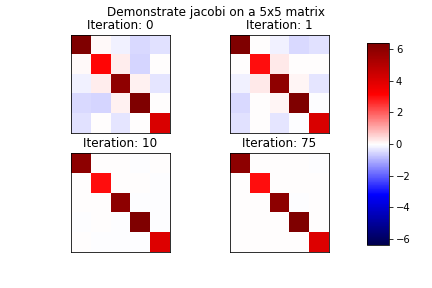
\includegraphics[scale=0.6]{../media/plots/jacobi.png}
\end{center}
\end{figure}


% ------------------------------------------------------------------------------
\subsection{QR-Method}

\begin{algorithm}[H]
\caption{\texttt{QRM1}}
\label{qr1-meth}
  \begin{algorithmic}
    \Require square matrix $A$
    \Statex \textbf{initialize: } $conv \gets False$
    \While{not $conv$}
      \State $Q, R \gets$ QR-Factorization of $A$
      \State $A \gets RQ$
      \If{$A$ is diagonal}
        \State $conv \gets \texttt{True}$
        \Statex
      \EndIf
    \EndWhile
    \Return $diag\left(A\right), Q$
  \end{algorithmic}
\end{algorithm}

\begin{figure}
\begin{center}
\caption{\href {https://github.com/thsis/NIS18/tree/master/media/plots}{Progress basic QR-Method}  \protect\includegraphics[scale=0.05]{qletlogo.pdf}}
  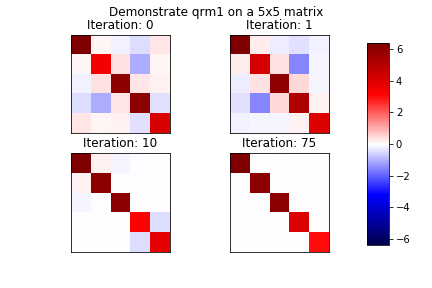
\includegraphics[scale=0.6]{../media/plots/qrm1.png}
\end{center}
\end{figure}


\subsubsection{Hessenberg Variant}


\begin{algorithm}[H]
\caption{\texttt{QRM2}}
\label{qr2-meth}
\begin{algorithmic}
  \Require square matrix $A$
  \State $A \gets \texttt{hessenberg(}A\texttt{)}$
  \State continue with: \Call {QRM1} A
\end{algorithmic}
\end{algorithm}

\begin{figure}
\begin{center}
\caption{\href {https://github.com/thsis/NIS18/tree/master/media/plots}{Progress Hessenberg-QR-Method}  \protect\includegraphics[scale=0.05]{qletlogo.pdf}}
  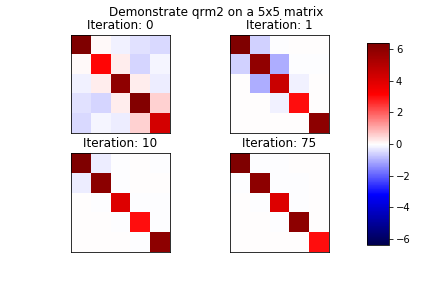
\includegraphics[scale=0.6]{../media/plots/qrm2.png}
\end{center}
\end{figure}


\subsubsection{Accelerated Variant}

\begin{algorithm}[H]
\begin{algorithmic}
\caption{\texttt{QRM3}}
\Require square matrix $A \in \mathbb{R}^{p \times p}$
\State $T \gets \texttt{hessenberg}(A),\ conv \gets False$
\While{not $conv$}
    \State $Q, R \gets$ QR-Factorization of $T - t_{p-1, p-1} I$
    \State $T \gets RQ + t_{p-1, p-1}I$
    \If{$T$ is diagonal}
        \State $conv \gets True$
    \EndIf
\EndWhile
\Return $diag\left(T\right), Q$
\end{algorithmic}
\end{algorithm}

\begin{figure}
\begin{center}
\caption{\href {https://github.com/thsis/NIS18/tree/master/media/plots}{Progress Accelerated QR-Method}  \protect\includegraphics[scale=0.05]{qletlogo.pdf}}
  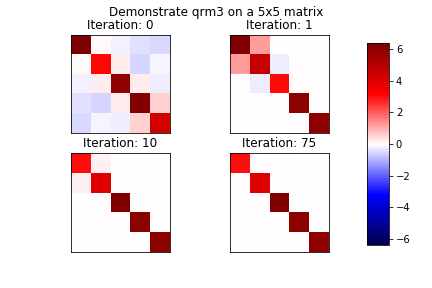
\includegraphics[scale=0.6]{../media/plots/qrm3.png}
\end{center}
\end{figure}

% ==============================================================================
\section{Analysis}

% ------------------------------------------------------------------------------
\subsection{Accuracy}

% ------------------------------------------------------------------------------
\subsection{Efficiency}

\begin{figure}
\begin{center}
\caption{\href {https://github.com/thsis/NIS18/blob/master/tests/tests_eigen.py}{Unit-tests: Iterations}  \protect\includegraphics[scale=0.05]{qletlogo.pdf}}
  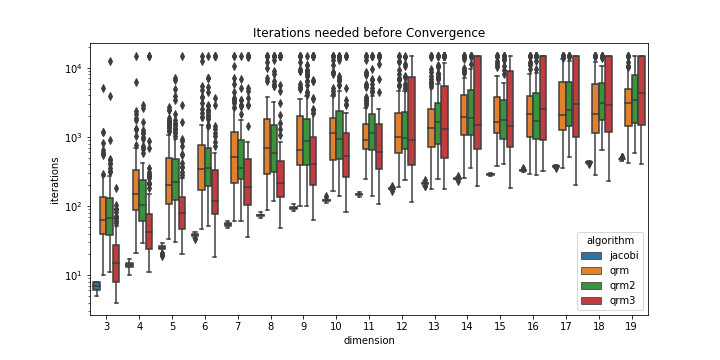
\includegraphics[width=\textwidth, height=5cm]{../media/plots/iterations_boxplot.png}
\end{center}
\end{figure}


% ==============================================================================
\section{Conclusion}
\begin{figure}
\caption{Decision process of final eigenvalue routine}
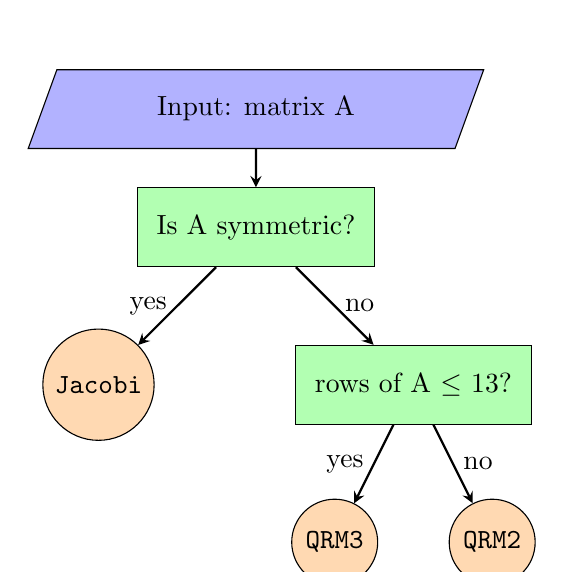
\begin{tikzpicture}
\node (in1) [io] {Input: matrix A};
\node (dec_sym) [decision, below of=in1, yshift=-0.5cm] {Is A symmetric?};
\node (algo1) [algo, below of=dec_sym, xshift=-2cm, yshift=-1cm] {\texttt{Jacobi}};
\node (dec_small) [decision, below of=dec_sym, xshift=2cm, yshift=-1cm] {rows of A $\leq$ 13?};
\node (algo2) [algo, below of=dec_small, xshift=-1cm, yshift=-1cm] {\texttt{QRM3}};
\node (algo3) [algo, below of=dec_small, xshift=1cm, yshift=-1cm] {\texttt{QRM2}};

\draw [arrow] (in1) -- (dec_sym);
\draw [arrow] (dec_sym) -- node[anchor=east] {yes} (algo1);
\draw [arrow] (dec_sym) -- node[anchor=west] {no} (dec_small);
\draw [arrow] (dec_small) -- node[anchor=east] {yes} (algo2);
\draw [arrow] (dec_small) -- node[anchor=west] {no} (algo3);
\end{tikzpicture}
\end{figure}
% ==============================================================================
\newpage
\section{Appendix}
\subsection{Eigenvalue Routines}
  \lstinputlisting[language=Python]{../algorithms/helpers.py}
  \lstinputlisting[language=Python]{../algorithms/eigen.py}

\subsection{Analysis: Figures}
  \lstinputlisting[language=Python]{../analysis/analysis.py}
    
\subsection{Analysis: Unit tests}
  \lstinputlisting[language=Python]{../tests/tests_eigen.py}
% ==============================================================================


\bibliographystyle{apalike}
\bibliography{references}

\end{document}